\subsection{Struktura wirtualnego efektora}
\label{subsec:ve-manip-struktura}

\begin{figure}[ht]
    \centering
    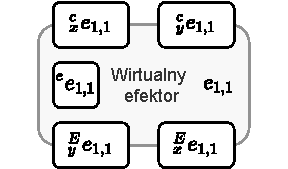
\includegraphics[width=0.75\columnwidth]{figures/ISR-ve-manip-model.pdf}
    \caption{Struktura ogólna wirtualnego efektora manipulatora sześciostopniowego}\
    \label{fig:model-ve-manip}
\end{figure}

Na rysunku~\ref{fig:model-ve-manip} przedstawiono widok wirtualnego efektora manipulatora w~systemie. Jego rolą jest nadzorowanie pracą rzeczywistego efektora sterującego ramieniem. Do poprawnej pracy podsystemu, wymagane są wszystkie cztery bufory komunikacyjne: dwa do obsługi rzeczywistego efektora oraz dwa do komunikacji z~podsystemem sterowania. Rozsądnym krokiem dyskretyzacji podsystemu jest zsynchronizowany z~pozostałymi podsystemami krok ${}^{e}T = \frac{1}{30}$s.

\subsubsection{Pamięć wewnętrzna}
W~pamięci wewnętrznej podsystemu przechowywane są ostatnie znane położenie końcówki robota we~współrzędnych kartezjańskich $\Theta_{\mathrm{ost}}$ oraz odpowiadająca mu konfiguracja stawów $q_{\mathrm{ost}}$.

\begin{equation}
    {}^{e}e_{1,1} = [q_{\mathrm{ost}}, \Theta_{\mathrm{ost}}]
\end{equation}

\subsubsection{Bufory komunikacyjne}
\begin{itemize}
    \item ${}^{c}_{x}e_{1,1} = \Theta_{\mathrm{zad}}$ - pozycja zadana końcówki we~współrzędnych kartezjańskich,
    \item ${}^{c}_{y}e_{1,1} = \Theta$ - aktualna pozycja końcówki we~współrzędnych kartezjańskich,
    \item ${}^{E}_{x}e_{1,1} = q$ - aktualna pozycja we~współrzędnych konfiguracyjnych,
    \item ${}^{E}_{y}e_{1,1} = q_{\mathrm{zad}}$ - zadana pozycja we~współrzędnych konfiguracyjnych.
\end{itemize}

\subsubsection{Funkcje pomocnicze}
Do poprawnego działania podsystemu, wymagana jest implementacja kilku funkcji pomocniczych, których konkretna definicja wymaga dokładnych parametrów omawianego manipulatora.

\begin{itemize}
    \item \texttt{FK($q$)} - kinematyka prosta, pozwala obliczyć pozycję końcówki robota w~przestrzeni kartezjańskiej, korzystając z~wiedzy na temat pozycji stawów robota,
    \item \texttt{IK($\Theta$)} - kinematyka odwrotna, pozwala obliczyć pozycję stawów, korzystając z~pozycji końcówki w~przestrzeni kartezjańskiej.
\end{itemize}

\subsection{Automat sterujący}
\begin{figure}[ht]
    \leftskip-3.5em
    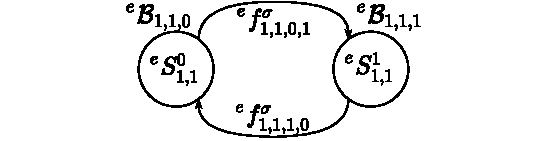
\includegraphics[width=1.3\columnwidth]{figures/ISR-ve-manip-behaviours.pdf}
    \caption{Automat zachowań wirtualnego efektora manipulatora sześciostopniowego}
    \label{fig:zachowania-ve-manip}
\end{figure}

Na rysunku~\ref{fig:zachowania-ve-manip} przedstawiony został automat sterujący wirtualnym efektorem manipulatora. Z~każdym z~dwóch stanów $ {}^{e}S_{1,1}^0,  {}^{e}S_{1,1}^1$ skojarzone zostało zachowanie ${}^{e}\mathcal{B}_{1,1,0}$ (\textbf{idle}) oraz ${}^{e}\mathcal{B}_{1,1,1}$ (\textbf{move}). 

Dla podanego podsystemu, nie ma potrzeby badać warunków rozłączności, ponieważ dla każdego stanu w~automacie, istnieje tylko jeden stan do którego można przejść. Z~racji że dla każdego $i$, ${}^{e}f^{\sigma}_{1,1,j,i} = \neg {}^{e}f^{\sigma}_{1,1,j,i}$, udowadnia to spełnienie warunku kompletność stanów następnych.

\subsection{Zachowanie idle}
\label{subsec:ve-manip-idle}

Zachowanie ${}^{e}\mathcal{B}_{1,1,0}$ (\textbf{idle}) opisuje aktywność manipulatora, w~trakcie gdy jego końcówka znajduje się w~pozycji zadanej oraz nie przychodzą żadne nowe polecenia od podsystemu sterowania. Gdy zachowanie to jest aktywne, manipulator stara się utrzymać ostatnią znaną, zadaną pozycję. 

\subsubsection{Funkcja przejścia}
\begin{equation}
    \begin{gathered}
        {}^{e_{1,1}, E_{1,1}}f_{1,1,0} \triangleq {}^{E}_{y}e_{1,1} = q_{\mathrm{ost}}\\
        {}^{e_{1,1}, c_{1,1}}f_{1,1,0} \triangleq {}^{c}_{y}e_{1,1} = \Theta_{\mathrm{ost}}
    \end{gathered}
\end{equation}

\begin{figure}[ht]
    \leftskip1.5em
    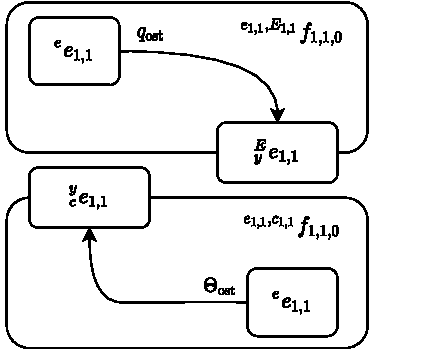
\includegraphics[width=\columnwidth]{figures/ISR-ve-manip-fp-idle.pdf}
    \label{fig:ve-manip-fp-idle}
    \caption{Zdekomponowana funkcja przejścia zachowania \textbf{idle} w~postaci DFD}
\end{figure}

\subsubsection{Warunki początkowe}
\begin{equation}
    {}^{e}f^{\sigma}_{1,1,1,0} \triangleq \Theta_{\mathrm{zad}} \neq \Theta
\end{equation}

\subsubsection{Warunki końcowe}
\begin{equation}
    {}^{e}f^{\tau}_{1,1,0} \triangleq \Theta_{\mathrm{zad}} = \Theta
\end{equation}

%%%%%%%%%%%%%%%%%%%%%%%%%%%%%%%%%%%%%%%%%%%%%%%%%%%%%%%%%%%%%%%%%%%%%%%%%%%%%%%%%%%

\subsection{Zachowanie move}
\label{subsec:ve-manip-move}

W~momencie przyjścia nowej pozycji zadanej końcówki manipulatora, aktywne staje się zachowanie ${}^{e}\mathcal{B}_{1,1,1}$, zwane dalej \textbf{move}. Na podstawie zadanej pozycji, obliczana jest kinematyka odwrotna, której wynikiem jest pozycja we~współrzędnych konfiguracyjnych, czyli wymagany kąt obrotu każdego ze~stawów manipulatora. Efektor zwraca również informację proprioreceptywną, w~postaci aktualnej pozycji końcówki robota, obliczanej za pomocą kinematyki prostej.

\subsubsection{Funkcja przejścia}
\begin{equation}
    \begin{gathered}
        {}^{e_{1,1}, E_{1,1}}f_{1,1,1} \triangleq {}^{E}_{y}e_{1,1} = IK(\Theta_{\mathrm{zad}})\\
        {}^{e_{1,1}, c_{1,1}}f_{1,1,1} \triangleq {}^{c}_{y}e_{1,1} = FK(q),\\
        {}^{e_{1,1}, e_{1,1}}f_{1,1,1} \triangleq {}^{e}e_{1,1} = [q, FK(q)]
    \end{gathered}
\end{equation}

\begin{figure}[ht]
    \leftskip-2em
    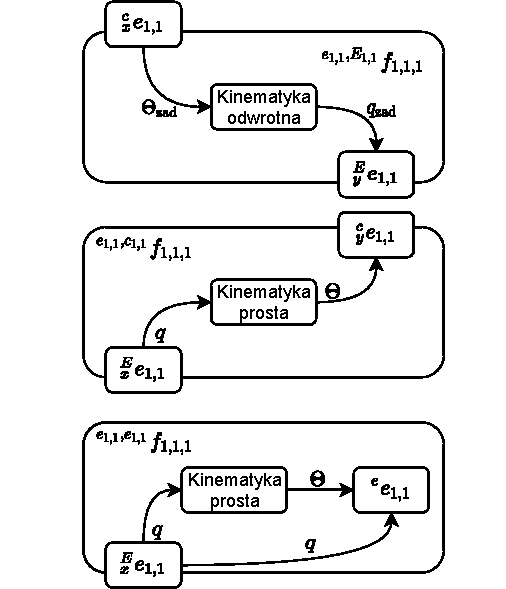
\includegraphics[width=1.1\columnwidth]{figures/ISR-ve-manip-fp-move.pdf}
    \caption{Zdekomponowana funkcja przejścia zachowania \textbf{move} w~postaci DFD}
    \label{fig:ve-manip-fp-move}
\end{figure}

\subsubsection{Warunki początkowe}
\begin{equation}
    {}^{e}f^{\sigma}_{1,1,0,1} \triangleq \Theta_{\mathrm{zad}} \Theta
\end{equation}

\subsubsection{Warunki końcowe}
\begin{equation}
    {}^{e}f^{\tau}_{1,1,1} \triangleq \Theta_{\mathrm{zad}} = \Theta
\end{equation}

%%%%%%%%%%%%%%%%%%%%%%%%%%%%%%%%%%%%%%%%%%%%%%%%%%%%%%%%%%%%%%%%%%%%%%%%%%%%%%%%%%%
